% $Id: header.tex 1229 2009-10-23 13:58:42Z inf6254 $
%%%%%%%%%%%%%%%%%%%%%%%%%%%%%%%%%%%%%%%%%%%%%%%%%%%%%%%%%%%%%%%%%%%%%%%
\documentclass
  [ %twoside            % beidseitiger Druck
  , openright          % Kapitel beginnen auf einer rechten Seite
  , listof=totoc       % Verzeichnisse im Inhaltsverzeichnis
  , bibliography=totoc % Literaturverzeichnis im Inhaltsverzeichnis
  , parskip=half       % Absätze durch einen vergrößerten Zeilenabstand getrennt
%  , draft              % Entwurfsversion
  ]{scrreprt}          % Dokumentenklasse: KOMA-Script Buch
  

%%%%%%%%%%%%%%%%%%%%%%%%%%%%%%%%%%%%%%%%%%%%%%%%%%%%%%%%%%%%%%%%%%%%%%%
% Packages
%%%%%%%%%%%%%%%%%%%%%%%%%%%%%%%%%%%%%%%%%%%%%%%%%%%%%%%%%%%%%%%%%%%%%%%
\usepackage{scrhack}

 
\usepackage{ifpdf}
\ifpdf
  \usepackage{ae}               % Fonts für pdfLaTeX, falls keine cm-super-Fonts installiert
  \usepackage{microtype}        % optischer Randausgleich, falls pdflatex verwandt
  \usepackage[pdftex]{graphicx} % Grafiken in pdfLaTeX
\else
  \usepackage[dvips]{graphicx}  % Grafiken und normales LaTeX
\fi

\usepackage[a4paper,%
            inner=2.0cm,outer=2.0cm,bindingoffset=0.5cm,%
            top=1.5cm,bottom=1.5cm,%
            footskip=1.0cm,includeheadfoot]{geometry}
            
\usepackage[utf8]{inputenc}         % Input encoding (allow direct use of special characters like "ä")
%\usepackage[english]{babel}
\usepackage[ngerman]{babel}
\usepackage[T1]{fontenc}
\usepackage[automark]{scrpage2} 	 % Schickerer Satzspiegel mit KOMA-Script
\usepackage{setspace}           	 % Allow the modification of the space between lines
\usepackage{booktabs}           	 % Netteres Tabellenlayout
\usepackage{multicol}               % Mehrspaltige Bereiche
\usepackage{quotchap}               % Beautiful chapter decoration
\usepackage[printonlyused]{acronym} % list of acronyms and abbreviations
\usepackage{subfig}                 % allow sub figures
\usepackage{tabularx}               % Tabellen mit fester Breite
\usepackage{lipsum}                 % für Blindtexte

% Layout
\pagestyle{scrheadings}
%\pagestyle{empty}
\clubpenalty = 10000
\widowpenalty = 10000
\displaywidowpenalty = 10000

\makeatletter
\renewcommand{\fps@figure}{htbp}
\makeatother

%% Document properties %%%%%%%%%%%%%%%%%%%%%%%%%%%%%%%%%%%%%%%%%%%%%%%%
\newcommand{\projname}{Der Projektname}
\newcommand{\titel}{Der Titel}
\newcommand{\authorname}{Max Mustermann}
\newcommand{\thesisname}{Bachelor Thesis}
\newcommand{\untertitel}{untertitel }
\newcommand{\Datum}{26 Februar 2010}

\ifpdf
  \usepackage{hyperref}
  \definecolor{darkblue}{rgb}{0,0,.5}
  \hypersetup
  	{ colorlinks=true
  	, breaklinks=true
    , linkcolor=darkblue
    , menucolor=darkblue
    , urlcolor=darkblue
    , pdftitle={\projname -- \untertitel}
    , pdfsubject={\thesisname}
    , pdfauthor={\authorname}
    }
\else
\fi

\bibliographystyle{alpha}

%% Listings %%%%%%%%%%%%%%%%%%%%%%%%%%%%%%%%%%%%%%%%%%%%%%%%%%%%%%%%%
\usepackage{listings}
\KOMAoptions{listof=totoc} % necessary because of scrhack
\renewcommand{\lstlistlistingname}{List of Listings}
\lstset
  { basicstyle=\small\ttfamily
  , breaklines=true
  , captionpos=b
  , showstringspaces=false
  , keywordstyle={}
  }

\lstnewenvironment{inlinehaskell}
{\spacing{1}\lstset{language=haskell,nolol,aboveskip=\bigskipamount}}
{\endspacing}

\lstnewenvironment{inlinexml}
{\spacing{1}\lstset{language=XML,nolol,aboveskip=\bigskipamount}}
{\endspacing}

\newcommand{\haskellinput}[2][]{
  \begin{spacing}{1}
  \lstinputlisting[language=Haskell,nolol,aboveskip=\bigskipamount,#1]{#2}
  \end{spacing}
}

\newcommand{\haskellcode}[2][]{\mylisting[#1,language=Haskell]{#2}}

\newcommand{\mylisting}[2][]{
\begin{spacing}{1}
\lstinputlisting[frame=lines,aboveskip=2\bigskipamount,#1]{#2}
\end{spacing}
}

\begin{document}

\pagenumbering{Roman}

%%%%%%%%%%%%%%%%%%%%%%%%%%%%%%%%%%%%%%%%%%%%%%%%%%%%%%%%%%%%%%%%%%%

% Titelseite
\newgeometry{left=3cm,right=2cm,top=2.0cm,bottom=2.0cm}
\include{stuff/titelseite}
\restoregeometry

%%%%%%%%%%%%%%%%%%%%%%%%%%%%%%%%%%%%%%%%%%%%%%%%%%%%%%%%%%%%%%%%%%%

% Mehr Platz für Nummerierung benötigt in Verzeichnissen, wenn ein Kapitel 10 oder mehr Bilder hat
\DeclareTOCStyleEntry[numwidth=3em]{tocline}{figure} % Für Abbildungsverzeichnis
%\DeclareTOCStyleEntry[numwidth=3em]{tocline}{table} % Für Tabellenverzeichnis

\tableofcontents
\listoffigures
\listoftables
\cleardoublepage

%%%%%%%%%%%%%%%%%%%%%%%%%%%%%%%%%%%%%%%%%%%%%%%%%%%%%%%%%%%%%%%%%%%

\pagenumbering{arabic}

\begin{onehalfspace}

\begin{abstract}
\paragraphnl{Abstract}

{\small
Hier kommt gegebenenfalls ein Abstract hin, welches kurz die gesamte Arbeit inkl. dem Ergebnis zusammenfasst.

 Lorem ipsum dolor sit amet, consectetur adipiscing elit. Cras quis facilisis dui. Fusce pulvinar sagittis nibh vitae vehicula. Duis pulvinar egestas lacus non varius. Phasellus interdum interdum lectus, quis euismod neque viverra a. Aliquam erat volutpat. In felis felis, semper in ullamcorper vitae, commodo sed ipsum. Cras consequat lorem nibh. Duis vulputate tellus ante, eu porttitor tellus tempor ac. Praesent eget nisl condimentum, rhoncus magna sit amet, luctus ipsum. Nunc vestibulum condimentum turpis, ac finibus odio consectetur eu. Ut volutpat risus non sapien dignissim efficitur. Sed scelerisque metus at posuere condimentum. Vivamus finibus, neque et cursus malesuada, orci purus scelerisque arcu, ut sollicitudin neque mi eu massa. Pellentesque at luctus ipsum. Praesent eu hendrerit est. Sed blandit sem sem, vel condimentum lectus fermentum consectetur.

Sed quis sem vitae enim molestie dapibus. Sed sodales nulla luctus tristique porttitor. Nullam sit amet semper risus. Fusce mi purus, blandit vel felis et, placerat ultricies urna. Mauris pretium mi ac felis lacinia porta. Class aptent taciti sociosqu ad litora torquent per conubia nostra, per inceptos himenaeos. Curabitur sit amet turpis eget enim iaculis sollicitudin non non libero. Vestibulum auctor dictum sapien, vitae rutrum mauris. Aenean fringilla neque non risus vestibulum, a bibendum leo tempus. Nunc consectetur posuere neque non rutrum. Nullam volutpat mauris et ex pretium aliquam. 
}
\end{abstract}
\chapter{Einleitung}
\lipsum

\section{\"Uberblick}
\lipsum

\subsection{Spam}
\lipsum

\subsection{Eggs}
\lipsum

\section{Motivation}
\lipsum

\section{Ziel}
\lipsum

\section{Überblick über die Arbeit}
\lipsum
\chapter{Grundlagen}

In diesem Kapitel werden die Grundlagen der verwendeten Themen und Technologien --- Begriffe und Sachverhalte --- erläutert, die für das Verständnis der folgenden Arbeit notwendig sind.
Die Grundlagen werden ohne Bezug auf das konkrete Projekt, allgemein dargestellt. Sie sind zielgerichtet auf das Verständnis des Hauptteils bezogen.

% \paragraphnl ist ein custom command. Ein \paragraph plus ein line-break / new-line.
% (Nach \paragraphnl{Paragraph} muss eine Zeile frei gelassen werden.)

\section{Abschnitt\#1}

Lorem ipsum dolor sit amet, consectetur adipiscing elit. Integer efficitur ipsum ut nulla dignissim tincidunt. Nullam sit amet tempor urna. Ut euismod mattis orci, vel mattis mi malesuada in. 

\section{Abschnitt\#2}

Aliquam molestie fermentum vestibulum. Cras egestas molestie ipsum, vitae malesuada ante consectetur id. In turpis neque, pharetra eget neque vel, rhoncus tincidunt ex. 


\subsection{Unterabschnitt\#1}

Sed lacinia fermentum odio quis faucibus. Phasellus blandit orci vitae ipsum rutrum aliquam. 

\subsection{Unterabschnitt\#2}

Fusce ipsum nisl, luctus in interdum non, sodales sed lacus. 

\paragraphnl{Paragraph}

Fusce vitae fermentum tellus, vitae feugiat magna. 

\subsubsection{Unter-Unterabschnitt\#1}

Curabitur tincidunt mauris ac venenatis accumsan. 

\subsubsection{Unter-Unterabschnitt\#2}

Mauris efficitur sit amet mauris in sodales. 

\subsubsection{Unter-Unterabschnitt\#3}

Ut fringilla commodo sem, at commodo erat mattis sed. 

\subsection{Unterabschnitt\#3}

Integer aliquet orci nec ligula aliquam accumsan. 

\subsubsection{Unter-Unterabschnitt\#1}

Nullam auctor rhoncus ultrices. Nunc viverra consequat interdum. 

\subsubsection{Unter-Unterabschnitt\#2}

Integer venenatis convallis erat, sit amet elementum odio egestas interdum. 

\subsubsection{Unter-Unterabschnitt\#3}

Phasellus sagittis vestibulum libero vel sodales. 

\section{Abschnitt\#3}

Phasellus a facilisis felis, vel mollis velit. 

\subsection{Unterabschnitt\#1}

Quisque pulvinar turpis vitae bibendum condimentum. 

\subsection{Unterabschnitt\#2}

Nulla facilisi. Praesent iaculis euismod eros et consequat. Nullam efficitur facilisis sapien. 

\subsubsection{Unter-Unterabschnitt\#1}

Aenean non laoreet lectus. Phasellus tellus lorem, ullamcorper vel aliquam ut, sollicitudin accumsan nibh. 

\subsection{Unterabschnitt\#3}

Duis vel elementum justo. Proin sed enim ipsum. 

\chapter{Hauptkapitel\#1}

Jedes Kapitel sollte mit einer Kapiteleinleitung beginnen, die als Orientierungshilfe den Inhalt des Kapitels zusammenfasst und wesentliche Punkte hervorhebt.

Entwicklungsorientierte Abschlussarbeiten folgen im Hauptteil der Thesis häufig dem Phasenmodell des Software-Engineerings\footnote{Auch wenn die Arbeit (Erkenntnisse, Entwicklung, Programmierung, \ldots) in anderer
zeitlicher Reihenfolge gewonnen wurden, macht es aus didaktischen Gründen Sinn, dem Phasenmodell zu folgen, da es bekannt und üblich ist und so die Leser:innen die Arbeit leichter verstehen können.}, die jeweils in einem Kapitel ausgeführt werden können:
\begin{itemize}

\item Analyse\\
Die Analyse umfasst zwei wesentliche Fragestellungen: a) die \emph{Ist-Analyse} in der der vorgefundene Zustand dargelegt wird. b) die \emph{Anforderungs-Analyse} die die durch das Projekt umzusetzenden 
funktionalen und nicht-funktionalen Anforderungen erläutert.

\item Design (Entwurf)\\
Der Entwurf stellte die Architektur der Lösung und ihre grundsätzliche, informationstechnische Herangehensweise vor. 
Zentrales Element kann eine graphische Darstellung der beteiligten Komponenten und ihrer Interaktionen sein. Auch können benötigte Algorithmen auf abstrakter Ebene dargestellt werden.

\item Implementierung\\
Die Implementierung führt konkrete Programme oder Konfigurationen vor. Essentieller Programmcode, der die wesentlichen Herausforderungen umsetzte, wird in Auszügen diskutiert.

\item Test (Evaluation, praktischer Einsatz, Messungen)\\
Der Test führt das entstandene System im Einsatz, unter Echtweltbedingungen oder mit Hilfe synthetischer Daten, vor. Hier können ggf.\ auch Screenshots oder relevante Logs diskutiert werden.
\end{itemize}

% Dieses Kapitel konkretisiert die bereits genannten Problematiken, schildert und vergleicht mögliche Umsetzungsvarianten, um diese zu vergleichen und daraus eine Auswahl zu treffen.
Der Hauptteil kann und soll auf die in den Grundlagen vermittelten Begriffe und Sachverhalte zurückgreifen, um das Problem und seine Lösung in angemessener und möglichst verständlicher Weise zu beschreiben.

\section{weitere Layout--Beispiele}

\begin{table}[ht]
\centering
    \begin{tabular}{l r | r}
        \hline\hline
        \thead{Tabelle}
        &
        \thead{\# Einträge}
        &
        \thead{Proz. Anteil der\\ursprünglichen Einträge} \\ [0.5ex] 
        % \thead erlaubt Zeilenumbruch in header
        % [0.5ex] = Abstand zur nächsten Zeile
        \hline
        Face Position Orientation   & $\sim$ 67.847.000 (73.3 \%) &  100.0 \%\\
        Face Demographics           & $\sim$ 24.377.000 (26.3 \%) &   36.0 \%\\
        Image Details               &    $\sim$ 161.000 ( 0.2 \%) &    0.2 \%\\
        Face Details                &    $\sim$ 144.000 ( 0.2 \%) &    0.2 \%\\
        \hline
        \textbf{Gesamt}             &        92.528.750 (100 \%)  &  \\ [1ex]
        \hline\hline
    \end{tabular}
\caption{Verteilung der Einträge auf die gruppierten Tabellen}
\label{tab:verteilung}
\end{table}

\clearpage

\begin{wrapfigure}{l}{0.5\linewidth}
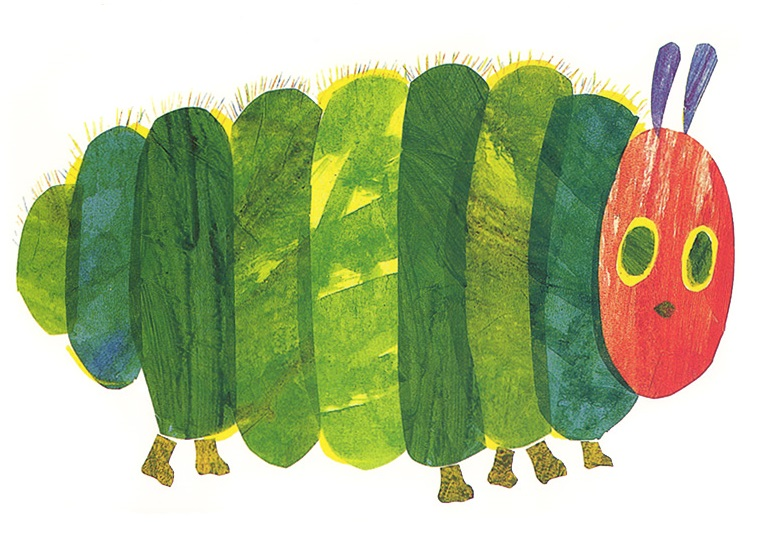
\includegraphics[width=\linewidth]{bilder/caterpillar.jpg}
\caption[Caterpillar]{Caterpillar\cite{caterpillar}}
\label{fig:caterpillar}
\end{wrapfigure}

Lorem ipsum dolor sit amet, consectetur adipiscing elit. Duis blandit, eros vel convallis scelerisque, ante risus hendrerit erat, id luctus urna velit in risus. Nunc nec viverra eros. Duis nisl mi, pharetra non massa ut, scelerisque scelerisque nisi. Donec faucibus nulla id risus condimentum viverra. Aliquam feugiat felis id massa tincidunt, nec malesuada lectus congue. Curabitur sagittis sapien ut augue cursus, eu congue purus sodales. 

Lorem ipsum dolor sit amet, consectetur adipiscing elit. Ut pulvinar viverra mollis. Proin magna justo, congue eget porta ut, maximus vel augue. Donec vehicula leo eu nisi vulputate blandit. Donec ultricies erat in eros suscipit, sit amet mattis elit vulputate. 

\begin{table}[hb]
\scriptsize
\begin{minipage}{0.49\linewidth}
\centering
\begin{tabular}{||c | r | r | r |} 
    \hline
    \textbf{Nr.} & \textbf{\# Ergeb.} & \textbf{PostgreSQL} & \textbf{MongoDB} \\ [0.5ex]
    \hline\hline
    \multirow{3}{*}{1.1} & \multirow{3}{*}{4.678} 
      & 0,9548 s & 0,3056 s \\
    & & 0,8997 s & 0,1290 s \\
    & & 0,9101 s & 0,1213 s \\
    \hline
    \multirow{3}{*}{1.2} & \multirow{3}{*}{4.678} 
      & 1,1088 s & -- \\
    & & 1,2218 s & -- \\
    & & 1,2137 s & -- \\
    \hline
    \multirow{3}{*}{1.3} & \multirow{3}{*}{4.678} 
      & 0,0403 s & -- \\
    & & 0,0412 s & -- \\
    & & 0,0401 s & -- \\
    \hline
    \multirow{3}{*}{2} & \multirow{3}{*}{4.678} 
      & 0,9498 s & 0,1466 s \\
    & & 0,9729 s & 0,1083 s \\
    & & 0,9071 s & 0,1066 s \\
    \hline
    \multirow{3}{*}{3} & \multirow{3}{*}{10.043} 
      & 0,2779 s & 0,3600 s \\
    & & 0,3079 s & 0,2429 s \\
    & & 0,2992 s & 0,2498 s \\
    \hline
    \multirow{3}{*}{4} & \multirow{3}{*}{2} 
      & 0,0018 s & 0,0727 s \\
    & & 0,0009 s & 0,0138 s \\
    & & 0,0009 s & 0,0070 s \\
    \hline
    \multirow{3}{*}{5} & \multirow{3}{*}{253.755}
      & 3,5117 s & 126,0782 s \\
    & & 3,4656 s & 106,1470 s \\
    & & 3,3282 s & 107,9439 s \\
    \hline
\end{tabular}
\end{minipage}
%
\begin{minipage}{0.49\linewidth}
\centering
\begin{tabular}{|c | r | r | r ||} 
    \hline
    \textbf{Nr.} & \textbf{\# Ergeb.} & \textbf{PostgreSQL} & \textbf{MongoDB} \\ [0.5ex] 
    \hline\hline 
    \multirow{3}{*}{6} & \multirow{3}{*}{5.141}
      & 2,1497 s & 12,1915 s \\
    & & 1,8485 s & 11,6134 s \\
    & & 1,7347 s & 11,2647 s \\
    \hline
    \multirow{3}{*}{7} & \multirow{3}{*}{694.907} 
      & 6,3388 s & 23,2439 s \\
    & & 6,6917 s & 22,4676 s \\
    & & 6,6002 s & 22,9043 s \\
    \hline
    \multirow{3}{*}{8} & \multirow{3}{*}{0} 
      & 0,0018 s & 0,0011 s \\
    & & 0,0008 s & 0,0009 s \\
    & & 0,0008 s & 0,0008 s \\
    \hline
    \multirow{3}{*}{9.1} & \multirow{3}{*}{1.635.965} 
      & 27,0328 s & 68,7589 s \\
    & & 28,4229 s & 58,9914 s \\
    & & 27,9176 s & 64,8253 s \\
    \hline
    \multirow{3}{*}{9.2} & \multirow{3}{*}{1.635.965} 
      & 12,2981 s & 73,4722 s \\
    & & 11,5675 s & 63,1674 s \\
    & & 11,4067 s & 68,5112 s \\
    \hline
    \multirow{3}{*}{10.1} & \multirow{3}{*}{14.222.062} 
      & 113,2476 s & 373,5514 s \\
    & & 107,6503 s & 370,8531 s \\
    & & 112,4459 s & 373,4111 s \\
    \hline
    \multirow{3}{*}{10.2} & \multirow{3}{*}{14.222.062} 
      & 143,6760 s & -- \\
    & & 141,0328 s & -- \\
    & & 142,5101 s & -- \\
    \hline
\end{tabular}
\end{minipage}
\caption{Beispieltabelle eines Benchmarks}
\label{tab:benchmark_results}
\end{table}

\chapter{Beispiel eines Code-Kapitels}

\section{Anforderungen}

Hier ein inline-codeblock: \lstinline[language=pseudo]{stop(); // Hammertime!}.\cite{tuoski:2022}

Oder so \lstinline[language=sql]{SELECT * FROM} wie hier.


\paragraphnl{Einfügen}

Aliquam molestie fermentum vestibulum. Cras egestas molestie ipsum, vitae malesuada ante consectetur id. 

\paragraphnl{Löschen}

In turpis neque, pharetra eget neque vel, rhoncus tincidunt ex. Sed lacinia fermentum odio quis faucibus. Phasellus blandit orci vitae ipsum rutrum aliquam. 

\paragraphnl{Ändern}

Fusce ipsum nisl, luctus in interdum non, sodales sed lacus. Fusce vitae fermentum tellus, vitae feugiat magna. 

\section{Implementierung}

Fusce luctus eros sem, id porttitor odio vestibulum sed. Etiam nisl eros, mollis rhoncus dolor vel, consectetur dignissim eros. Donec eu justo et ipsum posuere porttitor vitae quis lacus. 

\begin{wrapfigure}[26]{l}{0.5\linewidth}
% Sprache "sql" ist in header-datei definiert
\begin{lstlisting}[language=sql]
CREATE TABLE IF NOT EXISTS 
"Personen" (
    id serial NOT NULL,
    name text NOT NULL,
    geb_datum date NOT NULL,
    PRIMARY KEY (id)
);

CREATE OR REPLACE FUNCTION 
pruefe_alter()
    RETURNS TRIGGER
    LANGUAGE 'plpgsql'
AS $$
DECLARE
	alter_jahre int;
BEGIN
	SELECT date_part(
	    'year', 
	    age(NEW.geb_datum::TIMESTAMP))
	INTO alter_jahre;
	
	IF alter_jahre < 18 THEN
	    RAISE EXCEPTION 
	        'Person ist nicht volljaehrig';
	END IF;
	
	RETURN NEW;
END;
$$;
	
CREATE OR REPLACE TRIGGER 
trigger_person_einfügen
	BEFORE INSERT ON "Personen"
	FOR EACH ROW
	EXECUTE PROCEDURE pruefe_alter();
\end{lstlisting}
\captionsetup{type=figure}
\captionof{figure}{Beispiel einer\\Trigger-Definition}
\label{fig:trigger_example}
\end{wrapfigure}

Integer venenatis convallis erat, sit amet elementum odio egestas interdum. Phasellus sagittis vestibulum libero vel sodales. Phasellus a facilisis felis, vel mollis velit. Quisque pulvinar turpis vitae bibendum condimentum. Nulla facilisi. Praesent iaculis euismod eros et consequat. Nullam efficitur facilisis sapien. Aenean non laoreet lectus. Phasellus tellus lorem, ullamcorper vel aliquam ut, sollicitudin accumsan nibh. 

Fusce luctus eros sem, id porttitor odio vestibulum sed. Etiam nisl eros, mollis rhoncus dolor vel, consectetur dignissim eros. Donec eu justo et ipsum posuere porttitor vitae quis lacus. Duis convallis tellus non nibh ultrices, eget imperdiet metus iaculis. Integer non feugiat ante. Etiam felis massa, interdum eu egestas vel, eleifend id erat. In nec est ac orci elementum porttitor non non lorem. 

\clearpage

\subsection{Unterthema}

Vivamus quis lacus quis urna suscipit auctor. Nunc dignissim massa eu leo condimentum euismod. 

\subsection{Voraussetzungen}

Nunc mattis quis mauris a pharetra. Duis eu iaculis magna, id tristique dui. Duis sagittis mauris id elit maximus auctor. 

\subsection{Einfügen}

\paragraphnl{Einfügen aus Datei}

Pellentesque vitae ipsum elementum, iaculis enim mollis, fringilla sem. Integer eget odio porta, congue quam 

\subsection{Einfügen aus Webrequest}

Nulla imperdiet turpis in lorem eleifend aliquet sed ac libero. Morbi sed ultricies ipsum. 

\chapter{Zusammenfassung}
\appendix
\chapter{Anhang}

\vspace{-1cm}
\section{Unterteilung der Annotations-Attribute}
\label{sec:attribute_grouping}

\vspace{-1cm}
\begin{minipage}[t]{0.47\linewidth}
\begin{lstlisting}[language=json,title=Face Position Orientation]
{
    "bounding_box": {
        "position": {
            "x": int,
            "y": int
        }
        "width": int,
        "height": int
    },
    "eyes": {
        "left": {
            "x": int,
            "y": int
        },
        "right": {
            "x": int,
            "y": int
        }
    },
    "orientation": {
        "yaw": int,
        "pitch": int,
        "roll": int
    },
    "is_gaze_frontal": bool,
    "is_pose_ok": bool
}
\end{lstlisting}
\end{minipage}
%
\hspace{0.01\linewidth}
%
\begin{minipage}[t]{0.47\linewidth}
%
\begin{minipage}[t]{\linewidth}
\begin{lstlisting}[language=json,title=Image Details]
{
    "is_color_ok": bool,
    "is_exposure_ok": bool,
    "is_focus_ok": bool,
    "is_occluded": bool,
    "has_hotspots": bool,
    "has_shadows": bool,
    "has_red_eyes": bool
}
\end{lstlisting}
\end{minipage}
%
\begin{minipage}[t]{\linewidth}
\begin{lstlisting}[language=json,title=Face Demographics]
{
    "age": int,
    "age_estimated": int,
    "ethnicity": int,
    "gender": string
}
\end{lstlisting}
\end{minipage}
%
\begin{minipage}[t]{\linewidth}
\begin{lstlisting}[language=json,title=Face Details]
{
    "is_disguised": bool,
    "is_expression_neutral": bool,
    "eyes_open": bool,
    "has_facial_hair": bool,
    "mouth_closed": bool,
    "has_glasses": bool,
    "has_glasses_reflection": bool,
    "no_face_found": bool,
}
\end{lstlisting}
\end{minipage}
%
\end{minipage}

\clearpage

\begin{minipage}[t]{\linewidth}
\begin{lstlisting}[language=python,title=AnnotationSchema.py,firstnumber=34]
class AnnotationBase(BaseModel):
    age: StrictInt = None
    age_estimated: StrictInt = None
    gender: Gender = None
    ethnicity: StrictInt = None
    bounding_box: BoundingBox = None
    orientation: Orientation = None
    eyes: Eyes = None
    eyes_open: bool = None
    mouth_closed: bool = None
    is_disguised: bool = None
    is_expression_neutral: bool = None
    is_gaze_frontal: bool = None
    is_pose_ok: bool = None
    is_color_ok: bool = None
    is_exposure_ok: bool = None
    is_background_ok: bool = None
    is_focus_ok: bool = None
    is_occluded: bool = None
    has_hotspots: bool = None
    has_shadows: bool = None
    has_glasses: bool = None
    has_facial_hair: bool = None
    has_glasses_reflection: bool = None
    has_red_eyes: bool = None
    no_face_found: bool = None


class AnnotationAllowExtra(AnnotationBase, extra=Extra.allow):
    pass


class AnnotationForbidExtra(AnnotationBase, extra=Extra.forbid):
    pass
\end{lstlisting}
\end{minipage}

\end{onehalfspace}

%%%%%%%%%%%%%%%%%%%%%%%%%%%%%%%%%%%%%%%%%%%%%%%%%%%%%%%%%%%%%%%%%%%

\printbibliography{} % create with BibTeX

\chapter{Eidesstattliche Erklärung}
Ich erkl\"are hiermit an Eides statt, dass ich die vorliegende Arbeit selbstst\"andig und ohne Benutzung anderer als der angegebenen Hilfsmittel angefertigt habe; die aus fremden Quellen direkt oder indirekt \"ubernommenen Gedanken sind als solche kenntlich gemacht. Die Arbeit wurde bisher in \"ahnlicher Form keiner anderen Pr\"ufungskommission vorgelegt und auch nicht ver\"offentlicht.

\bigskip
\bigskip
\bigskip
\bigskip
	
   \begin{multicols}{2}
      \raggedright
      Ort, Datum
        
      \raggedleft
      \authorname
      
   \end{multicols}


\end{document}
